\documentclass[aspectratio=169,10pt]{beamer}
\usetheme[progressbar=frametitle,numbering=fraction]{metropolis}
\usepackage[spanish]{babel}
\usepackage[utf8]{inputenc}
\usepackage[T1]{fontenc}
\usepackage{lmodern}
\usepackage{booktabs,tikz,pgfplots,listings,xcolor,array,tabularx}
\usetikzlibrary{automata,positioning,arrows.meta}
\pgfplotsset{compat=1.18}
\definecolor{nuevo}{RGB}{220,110,10}
\definecolor{azul}{RGB}{50,80,140}
\setbeamercolor{alerted text}{fg=nuevo}
\setbeamercolor{frametitle}{bg=azul!90!black}
\setbeamercolor{progress bar}{fg=nuevo}
\lstdefinelanguage{Verilog}{morekeywords={assign,module,endmodule,input,output,wire,reg},sensitive=true,morecomment=[l]{//}}
\lstset{language=Verilog,basicstyle=\ttfamily\scriptsize,keywordstyle=\color{azul}\bfseries,backgroundcolor=\color{gray!8},frame=single,rulecolor=\color{gray!30},columns=fullflexible,keepspaces=true}
\newcommand{\sig}[1]{\texttt{#1}}

\title{Procesador RISC-V Dual-Issue\\ con BTB y predictor de 2 bits}
\subtitle{Proyecto 2 — Entrega final · Arquitectura de Computadoras}
\author{\small Alvarez Lovera, Sandra Sofia · Gutierrez Rodriguez, Mahir Gianpier · Alva Espinoza, Jose Luis}
\institute{UTEC · 2026 – 2}
\date{}

\begin{document}

\maketitle

\begin{frame}{Tres arquitecturas, mismos programas, mismo resultado}
\begin{columns}[T]
\column{0.55\textwidth}
\begin{itemize}
  \item \textbf{A — Pipeline Single-Issue:} 5 etapas, forwarding, stall por load-use y flush.
  \item \textbf{B — Dual-Issue in-order:} 2 vías, 2 ALU, Register File 4R/2W, 1 puerto de memoria y 1 unidad de saltos.
  \item \textbf{C — Dual-Issue + BTB:} predicción de saltos en Fetch.
\end{itemize}
\vspace{4pt}
Dos programas, sin modificaciones en ninguna versión:
\begin{itemize}
  \item el del profesor (312 instrucciones, etapas A–D);
  \item el propio (490 instrucciones, 4 etapas).
\end{itemize}
\column{0.42\textwidth}
\small
\begin{tabular}{lrrr}
\toprule
 & A & B & C \\
\midrule
\multicolumn{4}{l}{\textit{Programa del profesor}} \\
Ciclos & 458 & 387 & \alert{\textbf{292}} \\
IPC & 0.68 & 0.81 & \alert{\textbf{1.07}} \\
\midrule
\multicolumn{4}{l}{\textit{Programa propio}} \\
Ciclos & 583 & 437 & \alert{\textbf{373}} \\
IPC & 0.84 & 1.12 & \alert{\textbf{1.31}} \\
\bottomrule
\end{tabular}
\end{columns}
\end{frame}

\section{Arquitectura Dual-Issue}

\begin{frame}{Issue Unit: ¿salen dos, una o ninguna?}
\begin{columns}[T]
\column{0.5\textwidth}
La vía 1 lleva siempre la instrucción más antigua. El par sale completo salvo que haya:
\begin{itemize}
  \item \sig{RAWpar}: la 2.ª lee el \sig{rd} de la 1.ª;
  \item \sig{DosMem}: dos \sig{lw}/\sig{sw} (un solo puerto);
  \item \sig{DosSaltos}: dos \sig{beq}/\sig{jal} (una sola unidad).
\end{itemize}
Un load/store o un salto puede ir en \alert{cualquiera de las dos vías}: \sig{MemSelM} y \sig{BrSelE} asignan el recurso.
\column{0.47\textwidth}
\textbf{Reagrupamiento} si \sig{EmiteVia2 = 0}:
\begin{itemize}
  \item la vía 2 pendiente pasa a la vía 1;
  \item \sig{InstrF} entra como nueva vía 2;
  \item el PC avanza 4 en vez de 8;
  \item en E entra una burbuja en la vía 2.
\end{itemize}
\alert{Ninguna instrucción se pierde ni se repite}: las 3 versiones retiran exactamente 312 y 490 instrucciones.
\end{columns}
\end{frame}

\begin{frame}{Forwarding entre vías: WAW sobre x9 en el mismo par}
\centering
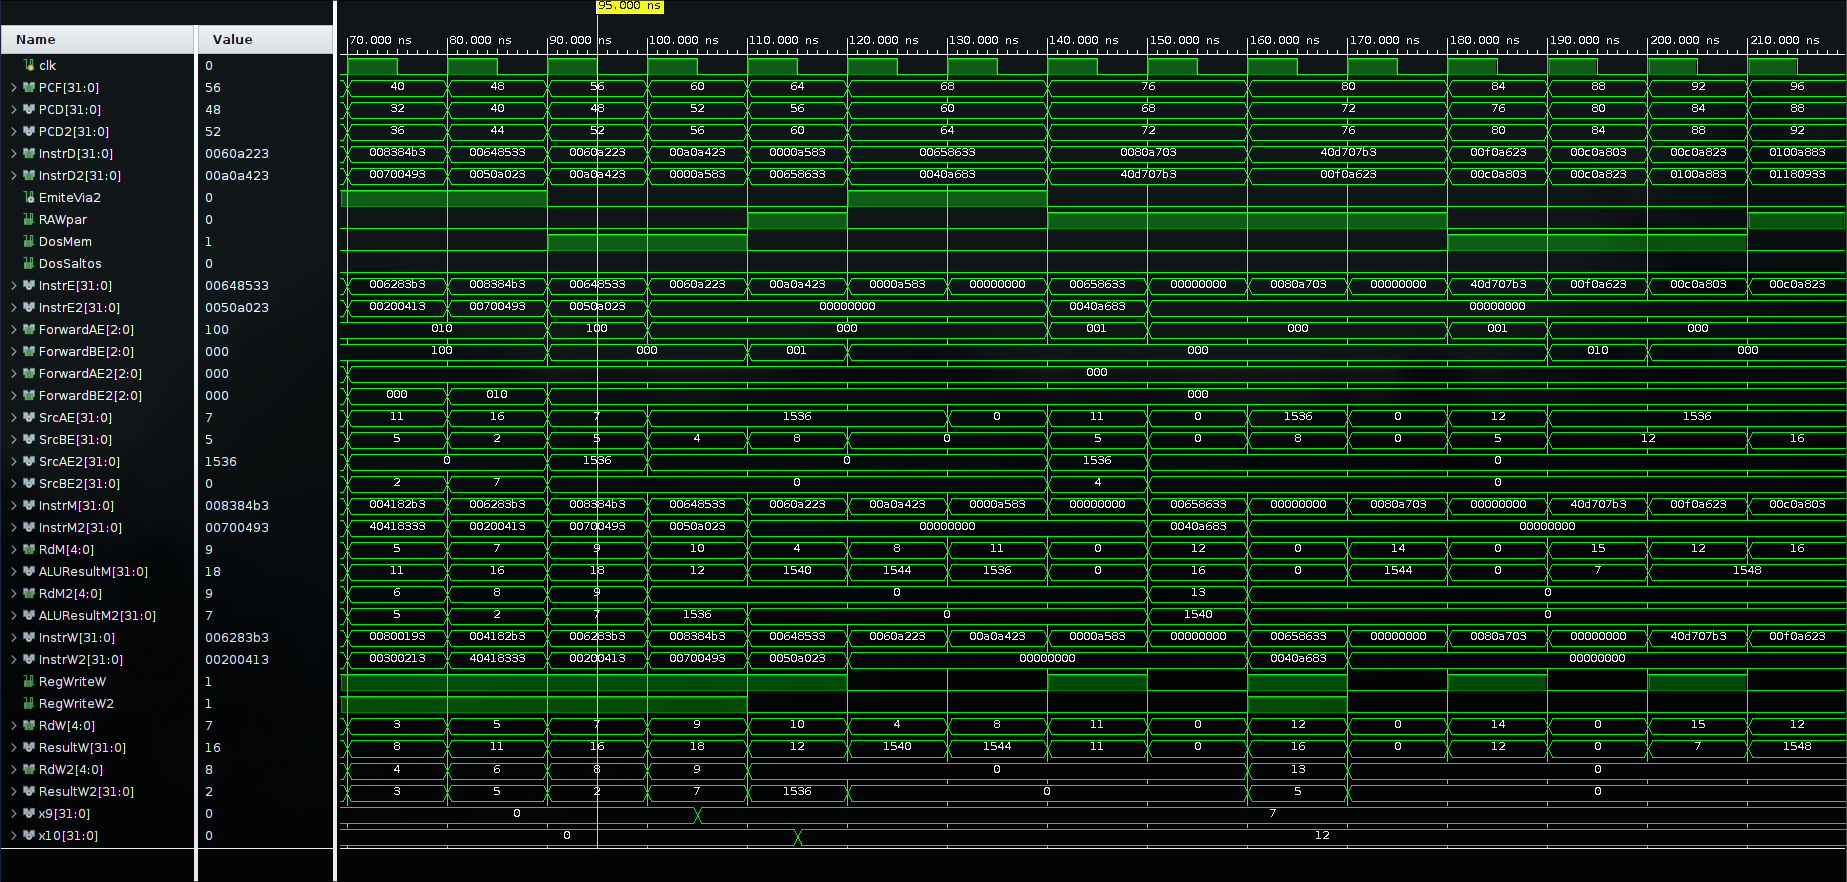
\includegraphics[width=0.93\textwidth,height=0.6\textheight,keepaspectratio]{capturas/w2_zoom.png}\\[2pt]
\footnotesize
\sig{add x9,x7,x8} y \sig{addi x9,x0,7} \alert{salen juntas} (sin RAW). En 95~ns, \sig{add x10,x9,x6} recibe \sig{ForwardAE = 100} y toma \sig{ALUResultM2 = 7}, de la vía 2 (la más joven).\\
Prioridad \textbf{M2 $>$ M1 $>$ W2 $>$ W1}; en WB se escriben las dos y queda la vía 2: x9 = 7, x10 = 12.
\end{frame}

\begin{frame}{Load-use en el Dual-Issue: el costo se duplica}
\centering
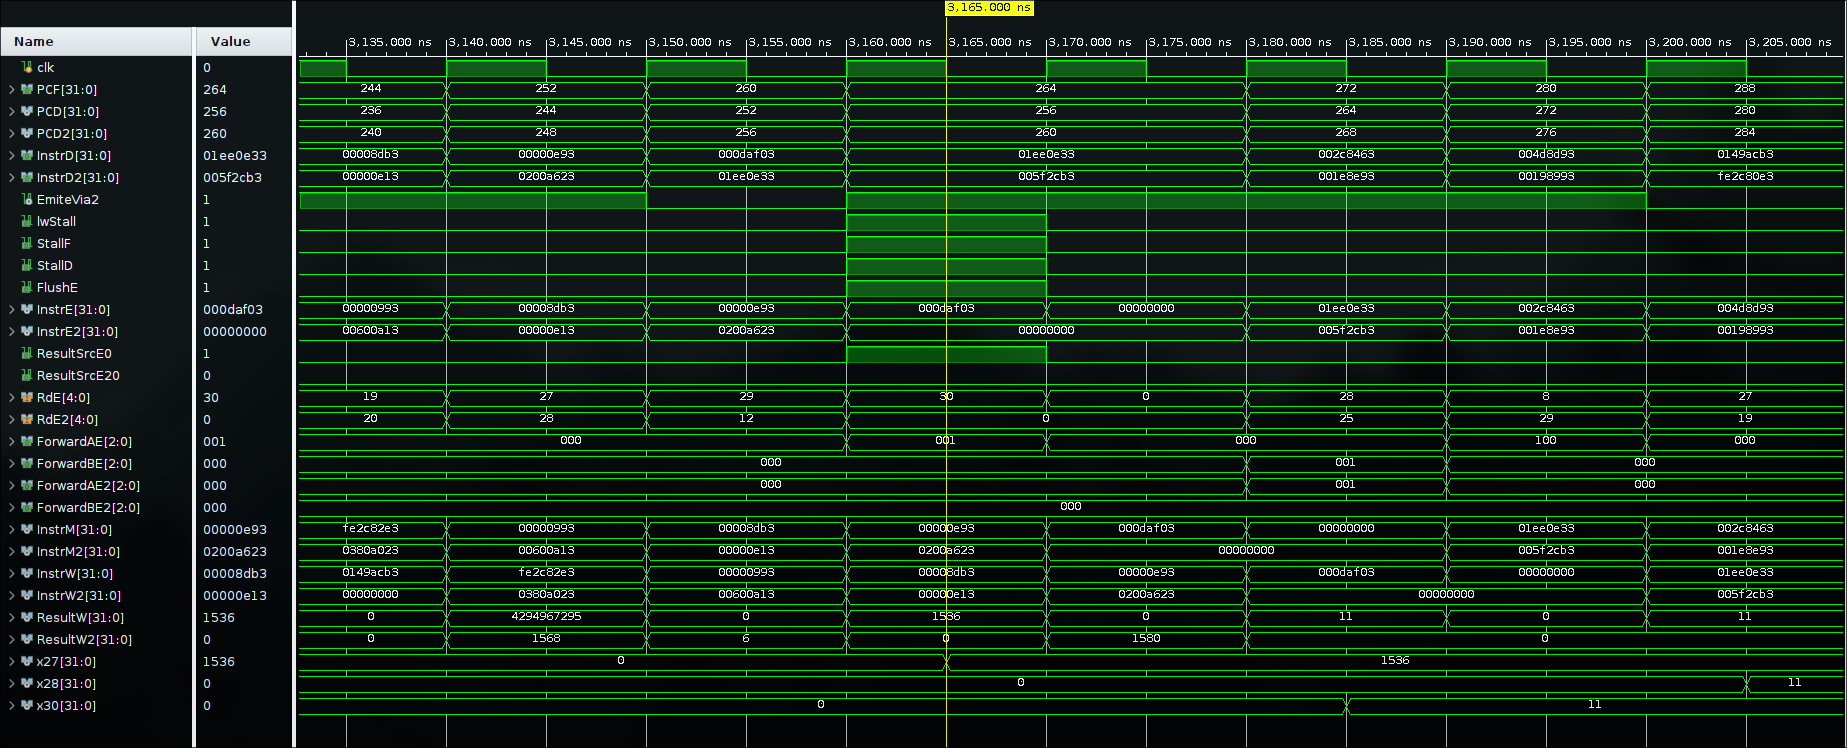
\includegraphics[width=0.93\textwidth,height=0.6\textheight,keepaspectratio]{capturas/w3_zoom.png}\\[2pt]
\footnotesize
\textbf{3155 ns:} RAW en el par (\sig{lw x30} | \sig{add x28,x28,x30}), sale solo el \sig{lw}.
\textbf{3165 ns:} \sig{lwStall} congela F/D y mete una burbuja en E.
\textbf{3185 ns:} \sig{ForwardBE = 001} y \sig{ForwardAE2 = 001}: un mismo productor alimenta a las dos vías.
\end{frame}

\section{Optimización: BTB + predictor de 2 bits}

\begin{frame}{Limitación medida: los saltos tomados}
\begin{columns}[T]
\column{0.52\textwidth}
\begin{itemize}
  \item En B, el salto se resuelve en \textbf{Execute}: si se toma, se anulan F y D.
  \item En Dual-Issue eso son \alert{2 ciclos × 2 slots = hasta 4 instrucciones} perdidas.
  \item Programa del profesor: 89 saltos ejecutados, \textbf{67 tomados}.
  \item La etapa C (puros lazos) ocupa 287 de los 387 ciclos de B, y ahí el Dual-Issue apenas supera al pipeline (287 frente a 330).
\end{itemize}
\column{0.45\textwidth}
\begin{tikzpicture}
\begin{axis}[xbar stacked, width=6.4cm, height=4.2cm, bar width=12pt, xmin=0,
  symbolic y coords={A,B}, ytick=data, xlabel={ciclos}, legend style={font=\tiny, at={(0.5,-0.42)}, anchor=north, legend columns=2, draw=none},
  every axis plot/.append style={draw=none}, tick label style={font=\scriptsize}, label style={font=\scriptsize}]
\addplot[fill=gray!50] coordinates {(31,A) (25,B)};
\addplot[fill=nuevo!80] coordinates {(330,A) (287,B)};
\addplot[fill=azul!50] coordinates {(97,A) (75,B)};
\legend{Etapas A+B, Etapa C (lazos), Etapa D}
\end{axis}
\end{tikzpicture}
\end{columns}
\end{frame}

\begin{frame}{Fundamento: predecir en Fetch, verificar en Execute}
\begin{columns}[c]
\column{0.5\textwidth}
\begin{itemize}
  \item \textbf{BTB:} 16 entradas de mapeo directo con valid, tag, \alert{target} y contador. Índice \sig{PC[5:2]}, tag \sig{PC[31:6]}.
  \item \textbf{Dos lecturas} por ciclo: \sig{PCF} y \sig{PCF+4} (los dos slots del paquete).
  \item \textbf{Contador de 2 bits:} predice tomado en 10 y 11. Tolera la única salida de un lazo.
  \item Si acierta, el salto cuesta \alert{0 ciclos}; si falla, lo mismo que en B.
\end{itemize}
\column{0.47\textwidth}
\centering
\begin{tikzpicture}[->,>={Stealth[length=2mm]}, node distance=1.45cm, every state/.style={minimum size=8mm, font=\scriptsize, thick}, font=\scriptsize]
  \node[state, fill=red!10] (s0) {00};
  \node[state, fill=red!5, right of=s0] (s1) {01};
  \node[state, fill=green!5, right of=s1] (s2) {10};
  \node[state, fill=green!10, right of=s2] (s3) {11};
  \path (s0) edge[bend left] node[above]{T} (s1) (s1) edge[bend left] node[above]{T} (s2) (s2) edge[bend left] node[above]{T} (s3)
        (s3) edge[bend left] node[below]{NT} (s2) (s2) edge[bend left] node[below]{NT} (s1) (s1) edge[bend left] node[below]{NT} (s0);
\end{tikzpicture}\\[6pt]
\scriptsize Entrada nueva: \sig{beq} en 10, \sig{jal} en 11.\\Solo se crea si el salto se toma.
\end{columns}
\end{frame}

\begin{frame}[plain]
\centering
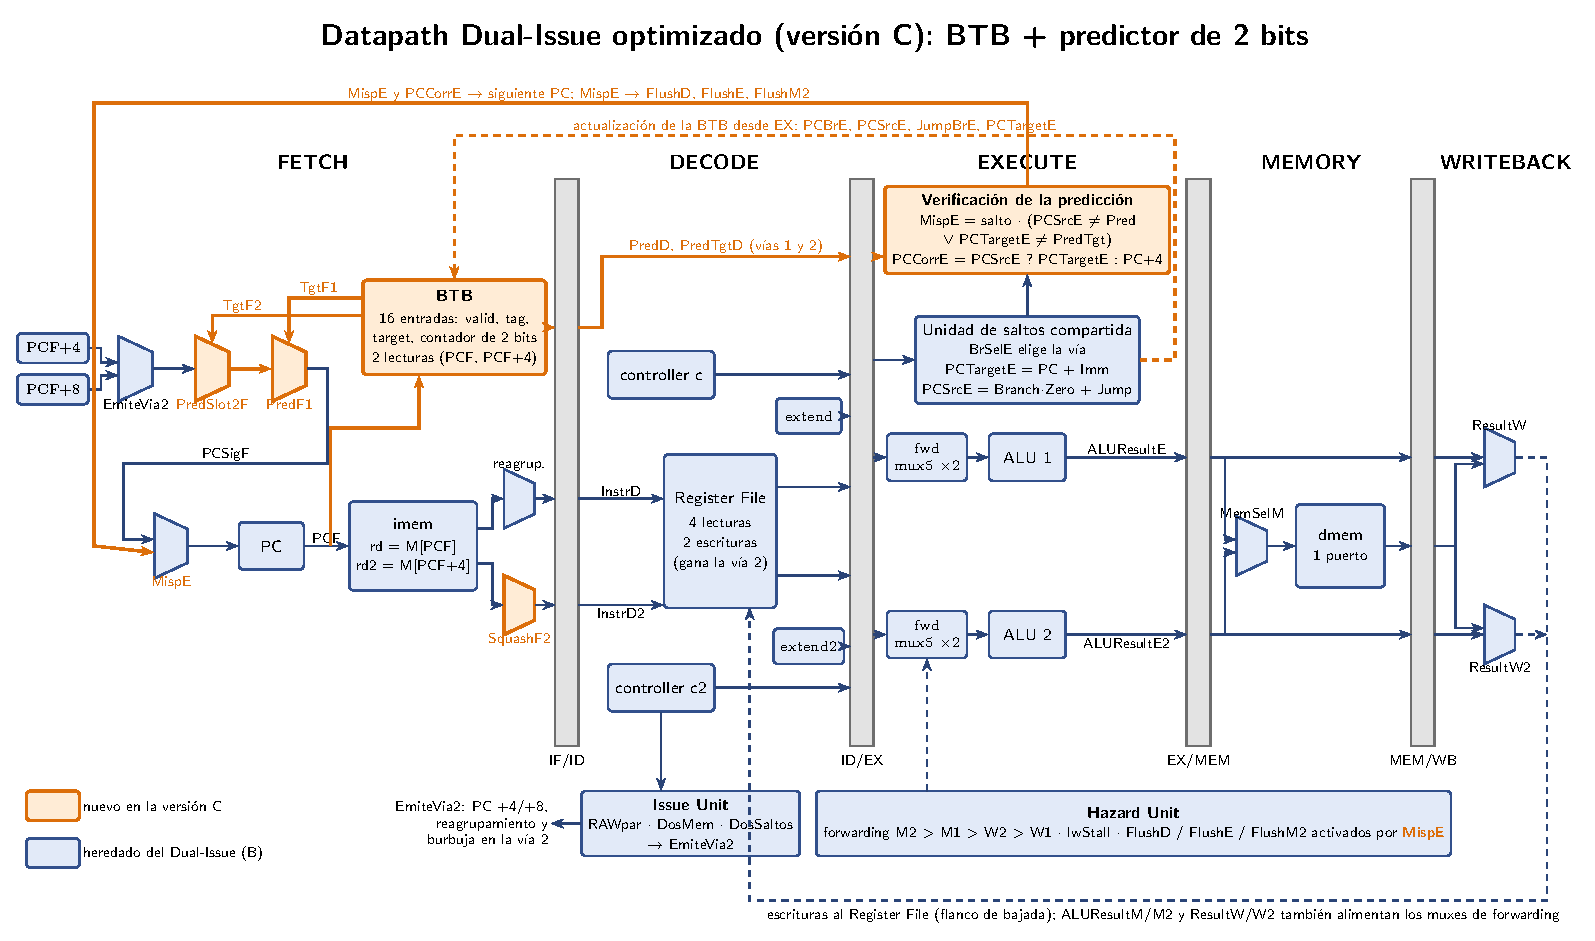
\includegraphics[width=\textwidth,height=0.97\textheight,keepaspectratio]{datapath_C.pdf}
\end{frame}

\begin{frame}[fragile]{Implementación: Fetch y Execute}
\begin{columns}[T]
\column{0.49\textwidth}
\textbf{Fetch:} siguiente PC según lo que realmente entra a Decode.
\begin{lstlisting}
assign SquashF2   = EmiteVia2 & PredF1;
assign PredSlot2F = EmiteVia2 & ~PredF1 & PredF2;
// PCSigF = PredF1 ? TgtF1 :
//          PredSlot2F ? TgtF2 :
//          EmiteVia2 ? PCF+8 : PCF+4
\end{lstlisting}
\footnotesize Si el slot 1 predice tomado, el slot 2 entra como burbuja. El reagrupamiento no necesita casos especiales: si el salto queda en la vía 2 de Decode, el fetch ya se redirigió.
\column{0.49\textwidth}
\textbf{Execute:} verificación en la unidad de saltos compartida.
\begin{lstlisting}
assign MispE = EsSaltoE &
   ((PCSrcE != PredBrE) |
    (PCSrcE & (PCTargetE != PredTgtBrE)));
// PCCorrE = PCSrcE ? PCTargetE : PC+4
\end{lstlisting}
\footnotesize \sig{FlushD/E/M2} pasan a depender de \sig{MispE}. Si el salto está en la vía 2, la vía 1 (más antigua) se conserva. El BTB se actualiza en el mismo ciclo.\\[3pt]
\textbf{Costo:} 976 bits de BTB + 132 FF de predicción.
\end{columns}
\end{frame}

\begin{frame}{Demostración: acierto y fallo del predictor}
\centering
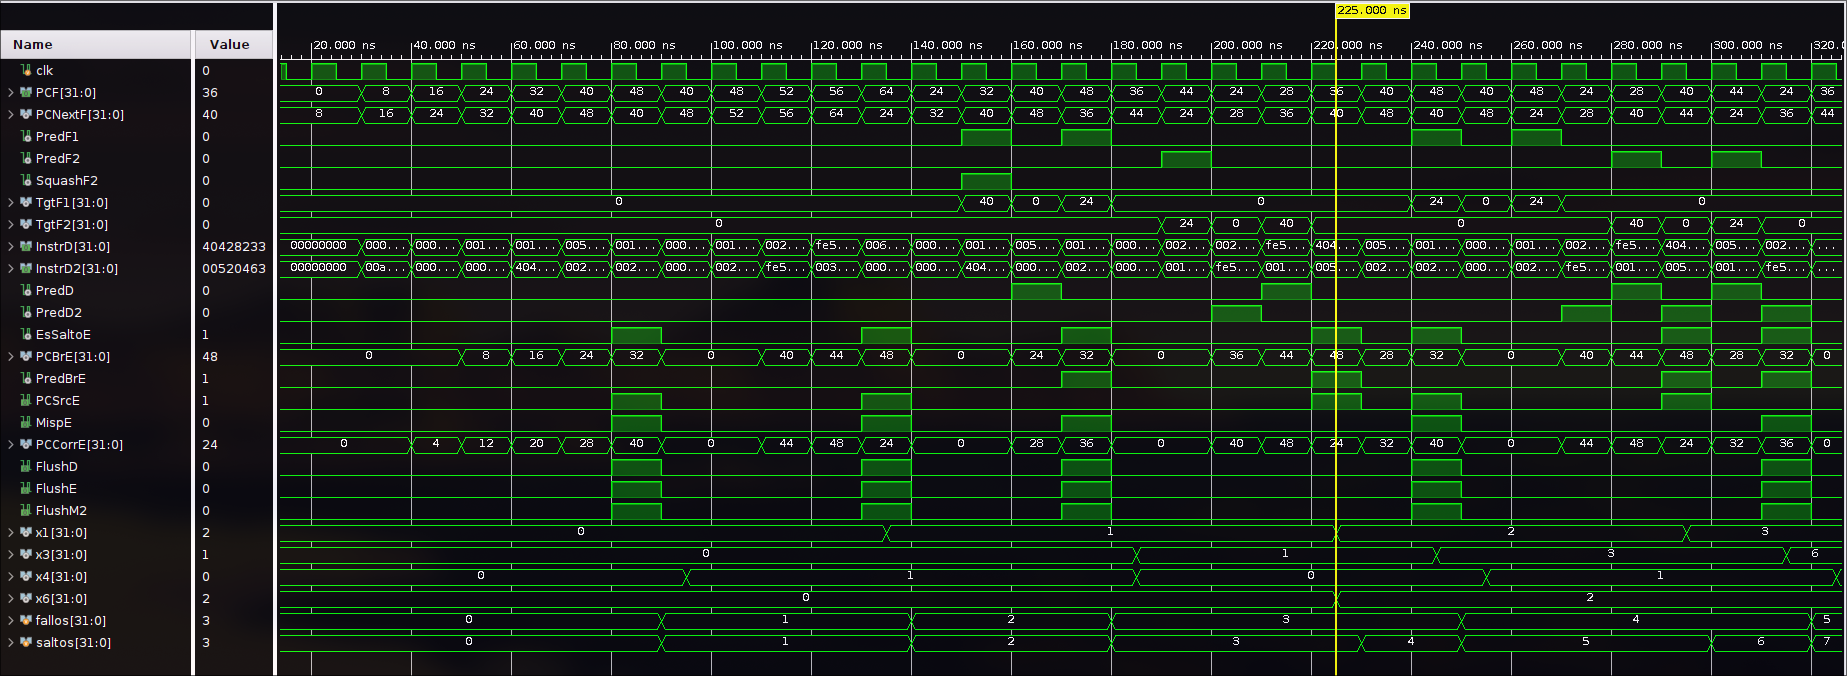
\includegraphics[width=0.93\textwidth,height=0.6\textheight,keepaspectratio]{capturas/w4_zoom.png}\\[2pt]
\footnotesize
\begin{tabular}{lccccl}
\toprule
Tiempo & PC & Pred & Tomado & \sig{MispE} & \\
\midrule
85 / 135 ns & 32 / 48 & 0 & 1 & 1 & fallo en frío \\
175 ns & 32 & 1 & 0 & 1 & salto alternante: falla \\
\alert{225 ns} & \alert{48} & \alert{1} & \alert{1} & \alert{0} & \alert{acierto en el lazo: no hay flush} \\
\bottomrule
\end{tabular}
\end{frame}

\section{Verificación y resultados}

\begin{frame}{Cómo verificamos}
\begin{columns}[T]
\column{0.5\textwidth}
\begin{itemize}
  \item \textbf{Modelo de commit} en el testbench: registros sombra actualizados en orden de programa en cada retiro. Checkpoint al final de cada etapa (\sig{chk\_X}, \sig{ok\_X}).
  \item \textbf{Mismo criterio de medición}: desde que baja \sig{reset} hasta el último retiro útil, sin el lazo \sig{fin}.
  \item \textbf{400 programas aleatorios}: A, B y C coinciden con un modelo ISA en Python.
  \item \textbf{Vivado 2025.2 (xsim)}: resultados idénticos ciclo a ciclo.
\end{itemize}
\column{0.47\textwidth}
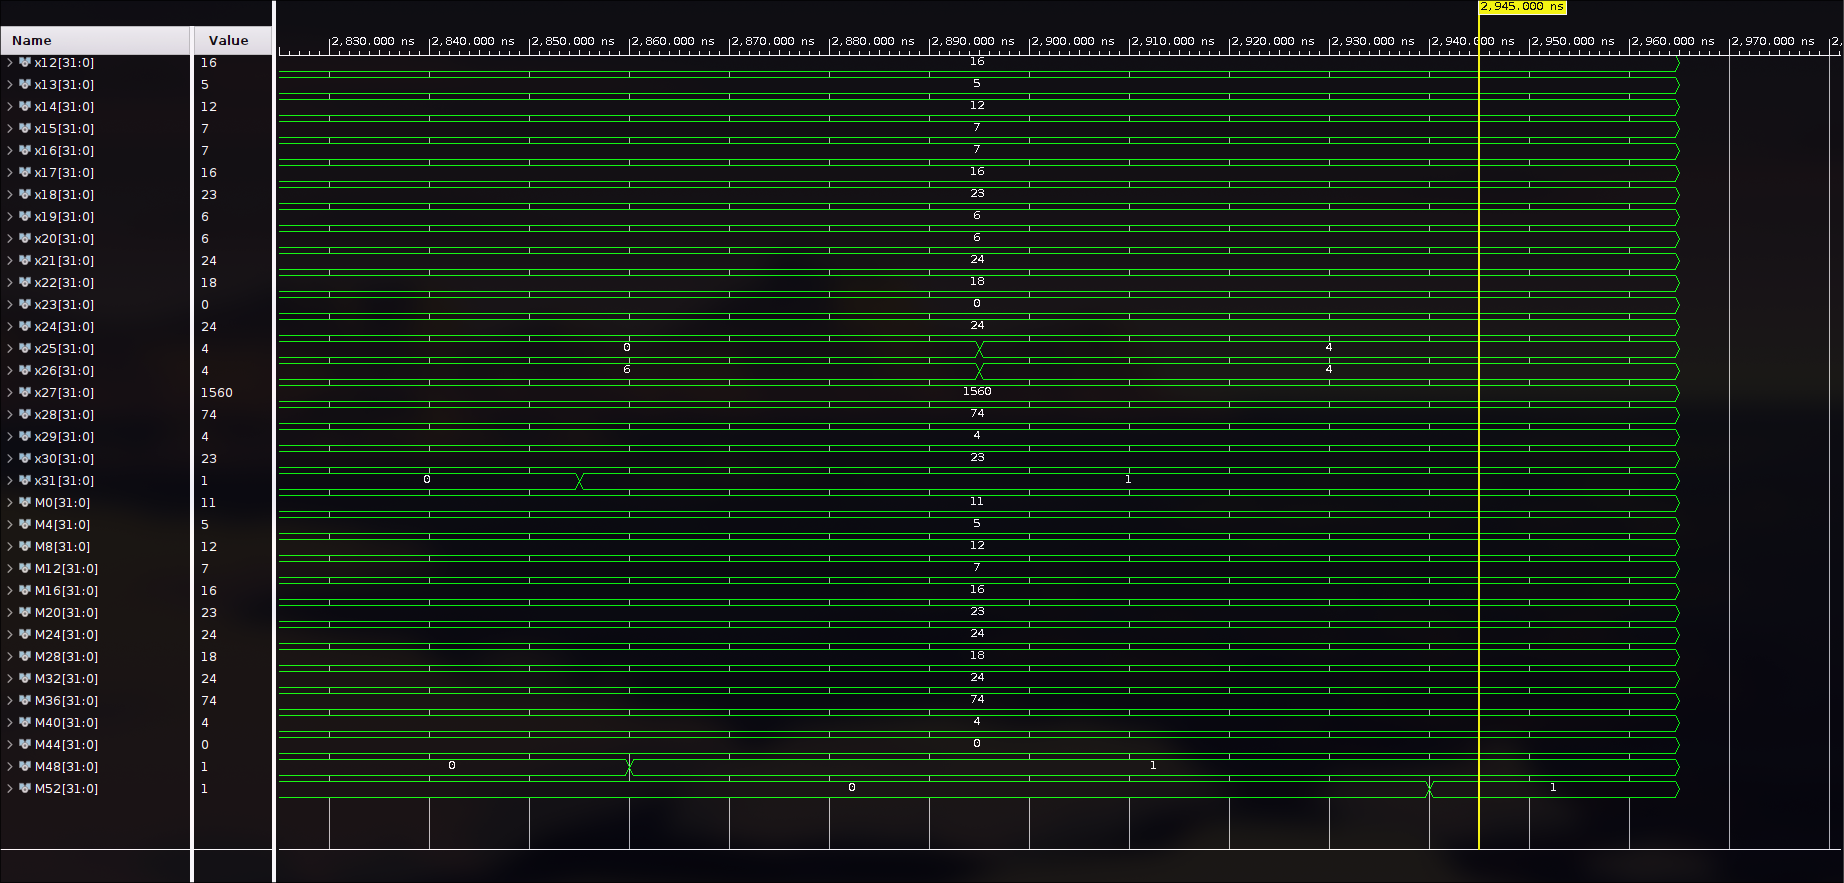
\includegraphics[width=\textwidth]{capturas/w1d_mem.png}\\
\scriptsize Cierre de la etapa D (2945 ns): x27 = 1560, x28 = 74, x29 = 4, x31 = 1, M36 = 74, M40 = 4, M52 = 1.\\[3pt]
\alert{Detalle:} en la etapa C, la última instrucción de C y la primera de D se retiran \emph{en el mismo paquete}.
\end{columns}
\end{frame}

\begin{frame}{Programa propio}
\begin{enumerate}
  \item \textbf{Inicialización con software pipelining:} \sig{addi} de la siguiente constante junto al \sig{sw} de la anterior, emitidas en pares.
  \item \textbf{Salto dependiente de datos:} \sig{B[i] = A[i] + i}, suma y conteo de \sig{A[i] > 7} con patrón irregular (\textit{N N T T N T N T …}).
  \item \textbf{Suma vectorial desenrollada ×2:} dos cadenas independientes, más ILP y salto de lazo predecible.
  \item \textbf{Lazos anidados 4×4:} suma por filas y máximo; el salto interno falla en cada salida.
\end{enumerate}
\vspace{4pt}
Resultado verificado: suma = 120, conteo = 8, filas = 68, 82, 104, 106 y máximo = 106.
\end{frame}

\begin{frame}{Comparación cuantitativa}
\centering
\small
\begin{tabular}{lrrr@{\hspace{16pt}}rrr}
\toprule
 & \multicolumn{3}{c}{Profesor} & \multicolumn{3}{c}{Propio} \\
\cmidrule(lr){2-4}\cmidrule(lr){5-7}
 & A & B & C & A & B & C \\
\midrule
Ciclos & 458 & 387 & \alert{292} & 583 & 437 & \alert{373} \\
Retiradas & 312 & 312 & 312 & 490 & 490 & 490 \\
CPI & 1.468 & 1.240 & \alert{0.936} & 1.190 & 0.892 & \alert{0.761} \\
IPC & 0.681 & 0.806 & \alert{1.068} & 0.840 & 1.121 & \alert{1.314} \\
Speedup vs.\ A & 1.00 & 1.18 & \alert{1.57} & 1.00 & 1.33 & \alert{1.56} \\
Speedup vs.\ B & — & 1.00 & \alert{1.33} & — & 1.00 & \alert{1.17} \\
\midrule
Flushes por salto & 68 & 68 & 33 & 46 & 46 & 25 \\
Stalls load-use & 9 & 11 & 12 & 0 & 48 & 41 \\
Ciclos con 2 retiros & 0 & 74 & 99 & 0 & 195 & 209 \\
Precisión predictor & — & — & 63\,\% & — & — & 62\,\% \\
\bottomrule
\end{tabular}
\end{frame}

\begin{frame}{¿Por qué no llegamos a IPC = 2?}
\begin{columns}[T]
\column{0.52\textwidth}
Cota estimada con un \textbf{predictor perfecto} y las mismas reglas de emisión:
\begin{center}
\small
\begin{tabular}{lccc}
\toprule
CPI & B & C & Perfecto \\
\midrule
Profesor & 1.24 & 0.94 & $\approx$0.81 \\
Propio & 0.89 & 0.76 & $\approx$0.66 \\
\bottomrule
\end{tabular}
\end{center}
C recorre el \alert{71\,\%} (profesor) y el \alert{57\,\%} (propio) de la distancia entre B y esa cota.
\column{0.45\textwidth}
\textbf{Límites estructurales:}
\begin{enumerate}
  \item RAW en el par: \sig{addi} → \sig{slt} → \sig{beq} en cada lazo.
  \item Un solo puerto de memoria (etapa B).
  \item Load-use: separa el par e inserta una burbuja.
  \item Un salto tomado en el slot 1 cierra el paquete.
\end{enumerate}
\footnotesize En el programa propio, A tiene 0 stalls load-use y B tiene 48: la distancia que basta en un pipeline escalar no basta con emisión doble.
\end{columns}
\end{frame}

\begin{frame}{¿Cuándo sirve la BTB y cuándo no?}
\begin{columns}[T]
\column{0.48\textwidth}
\textbf{Funciona bien}
\begin{itemize}
  \item Saltos de lazo: solo 2 fallos (frío y salida).
  \item \sig{jal}: solo falla la primera vez.
  \item Lazos C1, C2, C3 y D1: los flushes bajan de 68 a 33.
\end{itemize}
\column{0.48\textwidth}
\textbf{No funciona}
\begin{itemize}
  \item \alert{Patrón alternante}: \sig{beq x23,x2,C2a} falla 12 de 12; el contador oscila entre 01 y 10.
  \item Saltos que dependen de datos: \sig{A[i] > 7} falla 13 de 16.
  \item Código que se ejecuta una vez (D3–D6): fallos en frío.
  \item \alert{Puede empeorar un salto concreto}: C2a provoca 12 flushes en C frente a 6 en B.
\end{itemize}
\end{columns}
\end{frame}

\begin{frame}{Conclusiones y trabajo futuro}
\begin{itemize}
  \item Las 3 arquitecturas son \textbf{funcionalmente equivalentes}: checkpoints, testbenches de E2, 400 programas aleatorios y Vivado.
  \item El Dual-Issue mejora al pipeline entre \textbf{1.18×} y \textbf{1.33×}; lo frenan los saltos, las dependencias y el puerto único de memoria.
  \item La BTB elimina la mitad de los flushes: \alert{speedup de 1.57× y 1.56×} frente al pipeline, con \alert{IPC > 1} en los dos programas.
\end{itemize}
\vspace{4pt}
\textbf{Trabajo futuro}
\begin{itemize}
  \item Historia global (gshare) para patrones alternantes.
  \item Resolver los saltos en Decode: fallo de 1 ciclo.
  \item Instruction Queue para desacoplar Fetch de la emisión.
  \item Reordenamiento estático para separar los \sig{lw} de sus consumidores.
\end{itemize}
\end{frame}

\begin{frame}[standout]
¿Preguntas?
\end{frame}

\end{document}
